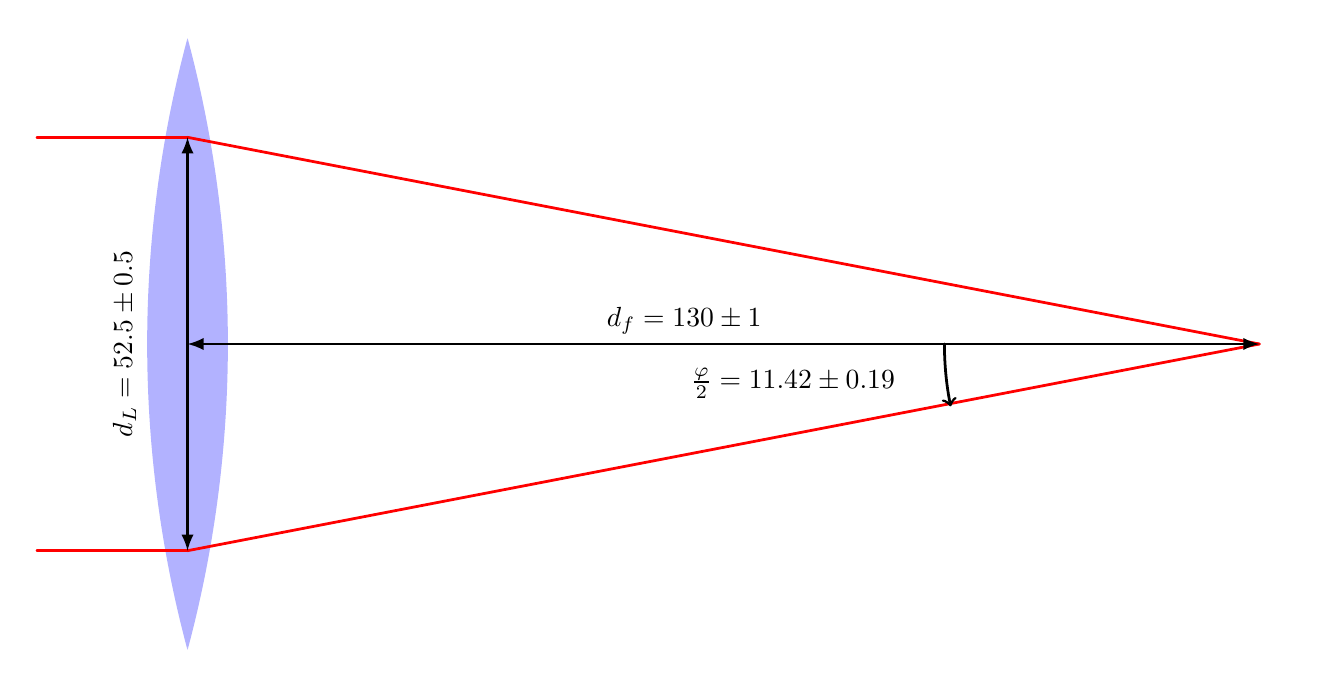
\begin{tikzpicture}
    \begin{scope}[x={(0mm,160mm)},y={(-40mm,40mm)},line width=1pt,cap=round]
        % bounding box
        \draw[white] (0mm,-40mm) rectangle (160mm,40mm);
        %\draw[-] (0mm,-30mm) -- (150mm,30mm);

        % Lens. Center: 20.125mm,0mm
        \fill[-,blue!30] (15mm,   0mm) -- (25.25mm,0mm) arc[start angle=0,  delta angle=15, radius=150mm] -- cycle;
        \fill[-,blue!30] (15mm,   0mm) -- (25.25mm,0mm) arc[start angle=0,  delta angle=-15,radius=150mm] -- cycle;
        \fill[-,blue!30] (25.25mm,0mm) -- (15mm,   0mm) arc[start angle=180,delta angle=15, radius=150mm] -- cycle;
        \fill[-,blue!30] (25.25mm,0mm) -- (15mm,   0mm) arc[start angle=180,delta angle=-15,radius=150mm] -- cycle;

        % incoming laser beams
        \draw[-,red] (1mm, 26.25mm) -- (20.125mm, 26.25mm);
        \draw[-,red] (1mm,-26.25mm) -- (20.125mm,-26.25mm);

        % outgoing laser beams
        \draw[-,red] (20.125mm, 26.25mm) -- (156.25mm,0mm);
        \draw[-,red] (20.125mm,-26.25mm) -- (156.25mm,0mm);

        % measurement arrow
        \draw[latex-latex,black] (20.125mm,0mm) -- (156.25mm,0mm);
        \draw[latex-latex,black] (20.125mm,-26.25mm) -- (20.125mm,26.25mm);
        \node[rotate=90] at (12.125mm,0mm) {$ d_L = \SI{52.5 \pm 0.5}{\milli\meter}$};
        \node at (83.2mm,3mm) {$ d_f = \SI{130 \pm 1}{\milli\meter}$};

        % angle arc
        \draw[->] (116.25mm,0mm) arc[start angle=180, delta angle=11.41, radius=40mm];
        \node at (97mm,-5mm) {$\frac{\varphi}{2} = \SI{11.42 \pm 0.19}{\degree}$};
    \end{scope}
\end{tikzpicture}
